% Generated by Sphinx.
\documentclass[letterpaper,10pt,english]{manual}
\usepackage[utf8]{inputenc}
\usepackage[T1]{fontenc}
\usepackage{babel}
\usepackage{times}
\usepackage[Bjarne]{fncychap}
\usepackage{sphinx}


\title{Lazyscripts Documentation}
\date{June 22, 2009}
\release{0.1}
\author{Hsin Yi Chen 陳信屹 (hychen)}
\newcommand{\sphinxlogo}{}
\renewcommand{\releasename}{Release}
\makeindex
\makemodindex
\newcommand\at{@}
\newcommand\lb{[}
\newcommand\rb{]}
\newcommand\PYGaz[1]{\textcolor[rgb]{0.00,0.63,0.00}{#1}}
\newcommand\PYGax[1]{\textcolor[rgb]{0.84,0.33,0.22}{\textbf{#1}}}
\newcommand\PYGay[1]{\textcolor[rgb]{0.00,0.44,0.13}{\textbf{#1}}}
\newcommand\PYGar[1]{\textcolor[rgb]{0.73,0.38,0.84}{#1}}
\newcommand\PYGas[1]{\textcolor[rgb]{0.25,0.44,0.63}{\textit{#1}}}
\newcommand\PYGap[1]{\textcolor[rgb]{0.00,0.44,0.13}{\textbf{#1}}}
\newcommand\PYGaq[1]{\textcolor[rgb]{0.38,0.68,0.84}{#1}}
\newcommand\PYGav[1]{\textcolor[rgb]{0.00,0.44,0.13}{\textbf{#1}}}
\newcommand\PYGaw[1]{\textcolor[rgb]{0.13,0.50,0.31}{#1}}
\newcommand\PYGat[1]{\textcolor[rgb]{0.73,0.38,0.84}{#1}}
\newcommand\PYGau[1]{\textcolor[rgb]{0.32,0.47,0.09}{#1}}
\newcommand\PYGaj[1]{\textcolor[rgb]{0.00,0.44,0.13}{#1}}
\newcommand\PYGak[1]{\textcolor[rgb]{0.14,0.33,0.53}{#1}}
\newcommand\PYGah[1]{\textcolor[rgb]{0.00,0.13,0.44}{\textbf{#1}}}
\newcommand\PYGai[1]{\textcolor[rgb]{0.73,0.38,0.84}{#1}}
\newcommand\PYGan[1]{\textcolor[rgb]{0.13,0.50,0.31}{#1}}
\newcommand\PYGao[1]{\textcolor[rgb]{0.25,0.44,0.63}{\textbf{#1}}}
\newcommand\PYGal[1]{\colorbox[rgb]{1.00,0.94,0.94}{\textcolor[rgb]{0.25,0.50,0.56}{#1}}}
\newcommand\PYGam[1]{\textbf{#1}}
\newcommand\PYGab[1]{\textit{#1}}
\newcommand\PYGac[1]{\textcolor[rgb]{0.25,0.44,0.63}{#1}}
\newcommand\PYGaa[1]{\textcolor[rgb]{0.19,0.19,0.19}{#1}}
\newcommand\PYGaf[1]{\textcolor[rgb]{0.25,0.50,0.56}{\textit{#1}}}
\newcommand\PYGag[1]{\textcolor[rgb]{0.13,0.50,0.31}{#1}}
\newcommand\PYGad[1]{\textcolor[rgb]{0.00,0.25,0.82}{#1}}
\newcommand\PYGae[1]{\textcolor[rgb]{0.13,0.50,0.31}{#1}}
\newcommand\PYGaZ[1]{\textcolor[rgb]{0.02,0.16,0.45}{\textbf{#1}}}
\newcommand\PYGbf[1]{\textcolor[rgb]{0.44,0.63,0.82}{\textit{#1}}}
\newcommand\PYGaX[1]{\textcolor[rgb]{0.00,0.44,0.13}{#1}}
\newcommand\PYGaY[1]{\textcolor[rgb]{0.25,0.44,0.63}{#1}}
\newcommand\PYGbc[1]{\textcolor[rgb]{0.25,0.44,0.63}{#1}}
\newcommand\PYGbb[1]{\textcolor[rgb]{0.78,0.36,0.04}{#1}}
\newcommand\PYGba[1]{\textcolor[rgb]{0.00,0.00,0.50}{\textbf{#1}}}
\newcommand\PYGaR[1]{\textcolor[rgb]{0.13,0.50,0.31}{#1}}
\newcommand\PYGaS[1]{\textcolor[rgb]{0.73,0.38,0.84}{#1}}
\newcommand\PYGaP[1]{\textcolor[rgb]{0.78,0.36,0.04}{\textbf{#1}}}
\newcommand\PYGaQ[1]{\textcolor[rgb]{0.25,0.44,0.63}{#1}}
\newcommand\PYGaV[1]{\textcolor[rgb]{0.05,0.52,0.71}{\textbf{#1}}}
\newcommand\PYGaW[1]{\textcolor[rgb]{0.25,0.44,0.63}{#1}}
\newcommand\PYGaT[1]{\textcolor[rgb]{0.13,0.50,0.31}{#1}}
\newcommand\PYGaU[1]{\textcolor[rgb]{0.25,0.50,0.56}{\textit{#1}}}
\newcommand\PYGaJ[1]{\textcolor[rgb]{0.56,0.13,0.00}{#1}}
\newcommand\PYGaK[1]{\textcolor[rgb]{0.25,0.44,0.63}{#1}}
\newcommand\PYGaH[1]{\textcolor[rgb]{0.50,0.00,0.50}{\textbf{#1}}}
\newcommand\PYGaI[1]{\fcolorbox[rgb]{1.00,0.00,0.00}{1,1,1}{#1}}
\newcommand\PYGaN[1]{\textcolor[rgb]{0.00,0.44,0.13}{#1}}
\newcommand\PYGaO[1]{\textcolor[rgb]{0.05,0.52,0.71}{\textbf{#1}}}
\newcommand\PYGaL[1]{\textcolor[rgb]{0.02,0.16,0.49}{#1}}
\newcommand\PYGaM[1]{\textcolor[rgb]{0.73,0.73,0.73}{#1}}
\newcommand\PYGaB[1]{\textcolor[rgb]{0.25,0.44,0.63}{#1}}
\newcommand\PYGaC[1]{\textcolor[rgb]{0.33,0.33,0.33}{\textbf{#1}}}
\newcommand\PYGaA[1]{\textcolor[rgb]{0.00,0.44,0.13}{#1}}
\newcommand\PYGaF[1]{\textcolor[rgb]{0.63,0.00,0.00}{#1}}
\newcommand\PYGaG[1]{\textcolor[rgb]{1.00,0.00,0.00}{#1}}
\newcommand\PYGaD[1]{\textcolor[rgb]{0.00,0.44,0.13}{\textbf{#1}}}
\newcommand\PYGaE[1]{\textcolor[rgb]{0.25,0.50,0.56}{\textit{#1}}}
\newcommand\PYGbg[1]{\textcolor[rgb]{0.00,0.44,0.13}{\textbf{#1}}}
\newcommand\PYGbe[1]{\textcolor[rgb]{0.00,0.44,0.13}{#1}}
\newcommand\PYGbd[1]{\textcolor[rgb]{0.40,0.40,0.40}{#1}}
\newcommand\PYGZat{@}
\newcommand\PYGZlb{[}
\newcommand\PYGZrb{]}

\begin{document}

\maketitle
\tableofcontents



內容:

\resetcurrentobjects


\chapter{Lazyscripts 0.1 多了什麼?}

本文件說明在2009年7月1號發行的 Lazyscripts 0.1版多了什麼新功能。

本文件會概括性介紹 Lazyscripts 0.1 發行版 ,但並不會詳細描述新功能,
欲知更多細節請閱讀 Lazyscripts 0.1 使用文件。


\section{與Lazybuntu最大的不同}
\begin{itemize}
\item {} 
不需頻繁更新主程式:
\begin{quote}

新版的Lazyscripts不再將 scripts與主程式合併釋出。Lazyscripts懶人包
只包含主程式,所有的功能會在執行時才從網路下載。而整個程式架構也分
成了使用者介面(GUI)、程式核心(Core)、以及功能(Scripts)。

功能將會隨著維護者的新增而更新,重新執行程式即可更新,不需要更新主
程式。
\end{quote}

\item {} 
用戶可隨意自訂Scripts:
\begin{quote}

如果您是進階使用者,未來Lazyscripts也提供幾個簡單步驟,讓您自訂專屬
於你自己的scripts。也就是說,使用者對於懶人包所連結的軟體選項,是可
以自由修改的。例如,您可以自行定義與客製化組合辦公室或班級內所需要的
Lazyscripts。這樣一份專屬的「軟體清單」懶人包,無疑造福更多的使用者。
\end{quote}

\end{itemize}


\section{全新的 Logo}

感謝 \href{http://pdtw.blogspot.com/}{Honkia}
為新生的Lazyscrtipts 設計Logo。


\section{更彈性化的系統架構}

現在的lazyscripts裡面的結構已經全部更新,現在變得更容易將客製化的腳本
(scripts)放入其中,下一個版本的 lazyscripts 可以更容易的置換腳本來源。


\section{自動更新腳本 (Script)}

Lazyscripts 全部的腳本 (script) 將會從網路上直接更新,當您每次執行
主程式時,都會從網路上自動下載最新的 scripts。


\section{新支援的Linux發行版本}

\begin{notice}{note}{Note:}
SuSE 以及 Fedora 支援正在開發中。
\end{notice}

0.1版開始支援 :
\begin{itemize}
\item {} 
Debian 5.0 (安裝桌面環境)

\item {} 
\href{http://news.ossacc.org/new\_icare\_readme\_linux/ezgo.html}{EzGo 自由軟體光碟}

\end{itemize}


\section{開發方式變更}
\begin{itemize}
\item {} 
程式碼採用Git管理

\item {} 
採用Google code作為專案管理工具

\item {} 
採用 Sphinix 作為文件撰寫工具
\begin{quote}

Sphinix 是 Python 2.6 版所採用的文件生成系統,使用 \href{http://docutils.sourceforge.net/rst.html}{reStructuredText}
語法處理文件內容關聯、排版,並且支援多種格式輸出,包含HTML、PDF、Latext。用 Sphinx 所生成的文件網站除了頁面能自訂樣式,自訂文件導覽順序,甚至還有附有搜尋功能。
\end{quote}

\end{itemize}


\strong{See Also:}

\begin{itemize}
\item {} 
\href{http://git-scm.org}{Git官網}

\item {} 
\href{http://sphinx.pocoo.org/index.html}{Sphinix 官網}

\end{itemize}



\resetcurrentobjects


\chapter{簡介}

Lazyscripts於2009年4月1日正式釋出,接替原本Lazybuntu的維護,
除了部份GUI的程式碼,及客製化Scripts仍延用外,核心架構及程式
碼幾乎全部改寫。

Lazybuntu 是由 PCMan 於 2007/09/25 發起,起因為 Ubuntu 雖然是
對初學者非常友善的 Linux 發行套件,但是仍然有許多未盡完美之處
,尤其在中文環境的方面,雖然 Ubuntu 的開發者花了不少功夫,仍然
不夠符合臺灣使用的習慣,預設的安裝也缺少一些國人常用的中文軟體。

此外,有些多媒體相關的軟體,因為某些法律上的爭議,和牽涉到一些專
利的問題,無法被 Ubuntu 官方套件收錄,但是這些套件卻是平日使用桌
面系統不可或缺的,例如 MP3 解碼,DVD 播放等重要功能,所以安裝好
Ubuntu 後,使用者往往還需要一番調校。

既然這些調教,是許多使用者裝好 Ubuntu 之後,第一件會想做的事情,
那與其讓初學者去搜尋文件看半天,為何不讓工具程式來代勞呢?在這樣
的想法之下,臺灣有許多網友,陸續提供了一些系統調校的小程式。 這些
小程式雖然解決了部份的問題,但是操作需要打指令,使用起來也不夠有
彈性。於是提供操作簡單的圖形介面,讓使用者只要動動滑鼠,在無需閱
讀文件或輸入指令的情況下,就可以輕鬆解決安裝後大部分的問題,便是
Lazybuntu 以及後來的 Lazyscripts 最重要的開發目的。

截至目前為止,Lazyscripts 支援 Ubuntu、Debian 等distrobution,可以
協助使用者設定網路、套件庫、設定好完善的中文環境、解決影音解碼、DVD
播放等各種常見問題、並安裝一些好用的常用軟體,將預設的 Linux 安裝,
調校成符合臺灣地區使用習慣的狀態。

而除了原本 Lazybuntu 擁有的功能外,Lazyscripts 更強化了客製化腳本
(Script)的管理方式,使Scripts 更容易分享、取得、合併,並且擁有更大
的彈性以應付依不同的客製目的。


\section{特色}
\begin{itemize}
\item {} 
不需頻繁更新主程式:
\begin{quote}

新版的Lazyscripts不再將 scripts與主程式合併釋出。Lazyscripts懶人包
只包含主程式,所有的功能會在執行時才從網路下載。而整個程式架構也分
成了使用者介面(GUI)、程式核心(Core)、以及功能(Scripts)。

功能將會隨著維護者的新增而更新,重新執行程式即可更新,不需要更新主
程式。
\end{quote}

\item {} 
用戶可隨意自訂Scripts:
\begin{quote}

如果您是進階使用者,未來Lazyscripts也提供幾個簡單步驟,讓您自訂專屬
於你自己的scripts。也就是說,使用者對於懶人包所連結的軟體選項,是可
以自由修改的。例如,您可以自行定義與客製化組合辦公室或班級內所需要的
Lazyscripts。這樣一份專屬的「軟體清單」懶人包,無疑造福更多的使用者。
\end{quote}

\end{itemize}


\section{系統需求}
\begin{itemize}
\item {} 
必須安裝
\begin{itemize}
\item {} 
GNU/Linux 發行套件
\begin{itemize}
\item {} 
Ubuntu 8.10 或 Ubuntu 9.04 桌面版本 AMD/x86

\item {} 
Debian Lenny 安裝標準桌面環境 (目前僅測試過 x86)

\end{itemize}

\item {} 
\href{http://git-scm.com/}{Git}

\item {} 
\href{http://www.python.org}{Python 2.6 以上}

\item {} 
\href{http://gitorious.org/projects/git-python/}{GitPython - Git Python Bidding Module}

\end{itemize}

\item {} 
開發者安裝
\begin{itemize}
\item {} 
\href{http://code.google.com/p/python-nose/}{Nose - Python Testing Framwork}

\item {} 
\href{http://www.gnu.org/software/automake/}{make - GNU make utility to maintain groups of programs}

\item {} 
\href{http://sphinx.pocoo.org/index.html}{Sphinix - Python Document Creator}

\end{itemize}

\end{itemize}


\section{如何安裝 Lazyscripts 主程式}

Lazyscripts 需要網路才可以使用,請務必確認您執行以下步驟時有網路連線可用。現在 Lazyscripts 提供與 lazybuntu 相同的簡易安裝方式。請先至以下網址:
\begin{itemize}
\item {} 
\href{http://code.google.com/p/lazyscripts/}{http://code.google.com/p/lazyscripts/}

\end{itemize}

右邊有個 Featured downloads 的區塊,請依照你的 CPU 架構選擇下載。如果你不知道你的 CPU 架構,請選擇 i386 版本。

下載完畢後,開啟檔案管理員到你下載的目錄,並且對壓縮檔按下右鍵,並且選擇『在此解壓縮』。解壓縮完畢後,會有一個 lazyscript 執行檔,雙擊執行即可。

如果您是第一次使用 Lazyscripts,必需要等待一段時間讓 Lazyscripts 安裝必要軟體,請耐心等候。待 Lazyscripts 使用介面出來後,即可勾選你需要的功能,並且按下確定執行。


\section{如何使用 Lazyscripts}

\begin{notice}{note}{Note:}
Lazyscripts 需要網路。
\end{notice}

簡單到不能再簡單的介面。

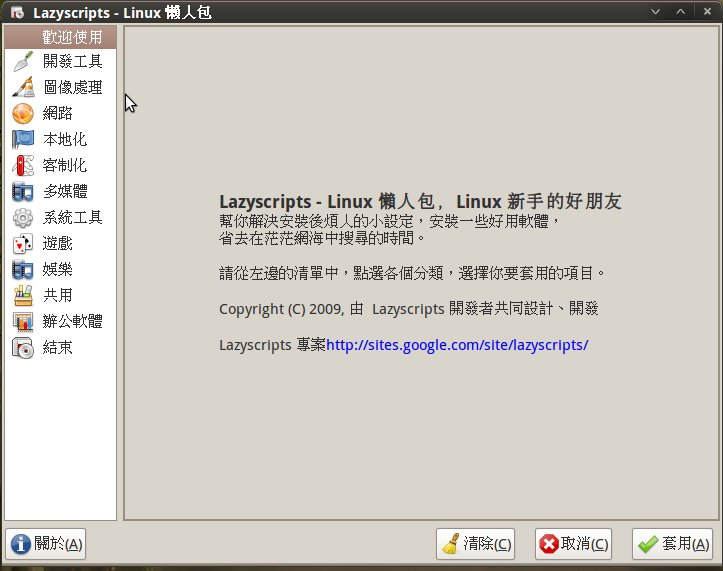
\includegraphics{userinterface.jpg}

只要下載 Lazyscripts,解壓縮,並雙擊後即可執行。接著只要依據軟體的分類屬性,適當地勾選您要安裝/不安裝的軟體選項,並按下最下方的套用鍵即可。畫面上的終端機(Terminal)就會幫您下載與安裝您所規劃組合的軟體套件,從安裝 Lazyscripts 到挑選軟體,到開始安裝選定的軟體,大約於 3 分鐘內應該可以完成

\resetcurrentobjects


\chapter{概念}

Lazyscripts 為延續 Lazybuntu 的易用性,在使用者介面上幾乎完全保留,
使用過Lazybuntu的使用者,除了進階功能,不需要再花心力學習新的操作方式。
而在介面下隱藏的卻是腳本散佈,控管的複雜設計,目前雖非盡善盡美,但已略達到原先設計初衷。

本章節將說明 Lazyscritps 的系統模型,魔鬼,都隱藏在細節裡。


\section{系統架構}

\begin{notice}{note}{Note:}
Lazyscripts Social Web 尚未開始實作!
\end{notice}

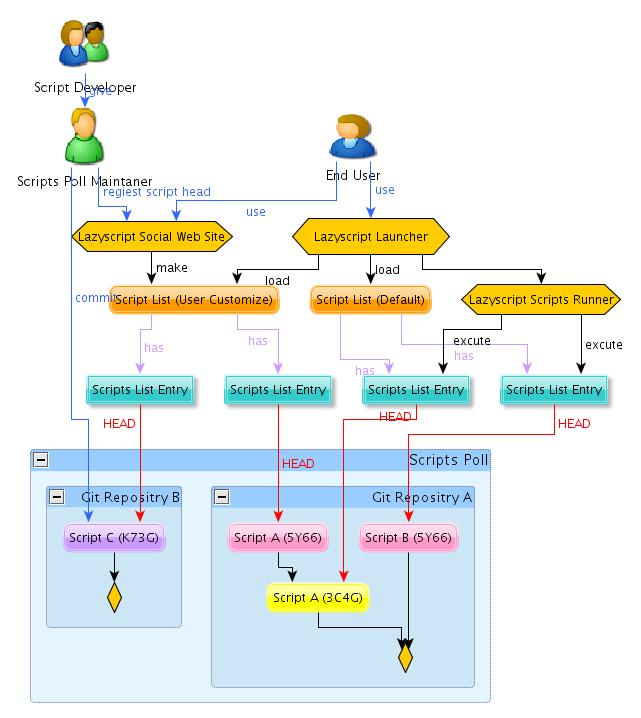
\includegraphics{lazyscripts_model.jpg}

\textbf{定義}

腳本 (Script)
\begin{quote}

安裝套件、客製作業系統。
\end{quote}

腳本庫 (Scritps Pool)
\begin{quote}

存放腳本。
\end{quote}

腳本清單 (Scripts List)
\begin{quote}

控制Lazyscritps可以使用的腳本版本。
\end{quote}

使用者 (End User)
\begin{quote}

使用Lazyscripts進行客製化安裝。
\end{quote}

腳本開發者 (Scripts Developer)
\begin{quote}

使用任何程式語言開發安裝或客制化腳本。
\end{quote}

腳本庫維護者 (Scripts Pool Mantainer)
\begin{quote}

接受、審核腳本提交,並製作Scripts List。
\end{quote}

主程式開發者 (Core Developer)
\begin{quote}

開發、修正主程式、文件撰寫。
\end{quote}


\section{腳本(Script)版本控制模型}


\section{腳本(Script)散佈模型}

\resetcurrentobjects


\chapter{腳本(Script)}


\section{如何撰寫腳本(Script)}

你需要一顆,虔誠的心…


\section{Script Category}
\begin{itemize}
\item {} 
Accessories – ex.

\item {} 
Productivity – ex. vim, openoffice

\item {} 
Graphics – ex.gimp

\item {} 
Development – ex. eclipse

\item {} 
Entertain – ex. mplayer,miro

\item {} 
InfoManagement – ex. sunbird, gnucash

\item {} 
Games – ex. gweled

\item {} 
Hardware – laptop customize script.

\item {} 
Multimedia – gstream

\item {} 
Networking – ex. firefox, pidgin, ie6, skype, pcman

\item {} 
System

\item {} 
Customize – 加快開機速度

\item {} 
Localization- 中文化環境

\end{itemize}


\section{Script Metadata}
\begin{itemize}
\item {} 
@name : script name.

\item {} 
@desc : script description.

\item {} 
@warn : script warning.

\item {} 
@category : script category id (defined by lazyscript team).

\item {} 
@maintaner : script maintaner.

\item {} 
@author : script author.

\item {} 
@license : script license.

\item {} 
@debian : script supports debian.

\item {} 
@ubuntu : script supports ubuntu.

\item {} 
@platform : support platform.

\item {} 
@child the : scripts need to run with

\item {} 
@hide : hide this item

\end{itemize}

\resetcurrentobjects


\chapter{腳本庫(Scripts Pool)}

容易更新,容易整合,可以做版本控管,而且速度要快!

這是 Lazyscritps 對客製化腳本儲存媒介的最基本要求。我們得承認,Linux 並不完美,
當安裝完後,並不像童話故事中的王子公主,從此過者美麗的生活,而是無盡調整的煩躁。

why need to get new version

why version control

why need merge easy


\section{官方腳本庫(Scritps Pool)}

要讓 Lazyscritps 支援不同的 Linux 發行版本很簡單,只要換掉腳本庫(Scritps Pool)
就好了,但前題是有人負責創建維護,各位有志之士,請拿出你的熱血來吧!!

以下為目前支援的發行版本:
\begin{itemize}
\item {} \begin{description}
\item[Ubuntu/Debian]\begin{itemize}
\item {} 
位置: git://github.com/billy3321/lazyscripts\_pool\_debian\_ubuntu.git

\item {} 
維護者:{}`Zhe-Wei Lin 林哲瑋 (billy3321,雨蒼) \textless{}\href{http://billy3321.blogspot.com/}{http://billy3321.blogspot.com/}\textgreater{}{}`\_ \textless{}billy3321 at gmail.com\textgreater{}

\end{itemize}

\end{description}

\item {} \begin{description}
\item[Ezgo 自由軟體光碟(Based On Ubuntu)]\begin{itemize}
\item {} 
位置: git://github.com/hychen/lazyscripts\_pool\_debian\_ubuntu.git

\item {} 
維護者:{}`Hsin Yi Chen 陳信屹 (hychen) \textless{}\href{http://hychen.wuweig.org}{http://hychen.wuweig.org}\textgreater{}{}`\_ \textless{}ossug.hychen at gmail.com\textgreater{}

\end{itemize}

\end{description}

\end{itemize}


\section{自訂腳本庫(Scritps Pool)}

TBD


\section{與上游腳本庫(Scripts Pool)同步}

TBD


\section{產生Scripts List}

TBD

\resetcurrentobjects


\chapter{如何幫忙}

著名的Linux開發者之一的雷蒙說過:「把使用者視為協同開發人,乃是迅速改善程式碼和有效除錯的最佳途徑!」Lazy 社群團隊一直保持與使用者的高度互動,誠摯希望使用者能透過任何管道告知我們使用狀況與建議。

你可以透過以下方式連繫我們。
\begin{enumerate}
\item {} 
IRC: irc.freenode.net \#lazyscripts

\item {} 
\href{http://groups.google.com/group/lazyscripts-dev/}{Lazyscripts Developer Mailing List}:

\item {} 
\href{http://hack.ingday.org}{HackingThursday 實體聚會}:
\begin{quote}

是一個台北由 Mat 發起的活動,Hychen 跟 Yuren 都會在這個活動中出現,歡迎當面遞送臭蟲。HacingThursday 每週四晚上會於特定咖啡店聚會。
\end{quote}

\item {} 
\href{http://kalug.linux.org.tw}{Kalug 實體聚會}:
\begin{quote}

KaLUG 是許多 Lazyscripts 開發者參與的聚會,包括Aminzai, Billy3321, Hychen, Yuren 都是此聚會的成員,而現在 Aminzai 與 Billy3321 (雨蒼) 會在這個聚會出現,如果您有臭蟲想親手遞交,請至 KaLUG 聚會 (高雄)。KaLUG 通常在每個月的第三個禮拜聚會。
\end{quote}

\end{enumerate}


\section{幫忙推廣}
\begin{itemize}
\item {} 
介紹給其他人

\item {} 
寫使用者文件

\item {} 
翻譯成其他語言

\end{itemize}


\section{回報臭蟲(Bug)}

Lazyscripts 懶人包目前採用 google code 作為問題回報系統。
若有任何問題請前往以下網址回報問題:
\begin{itemize}
\item {} 
\href{http://code.google.com/p/lazyscripts/issues/list}{http://code.google.com/p/lazyscripts/issues/list}

\end{itemize}

本專案接受中、英文問題回報,但採用英文為較理想。


\section{貢獻源碼}

你發現問題了嗎?歡迎直接修改源碼!Lazyscripts 懶人包現在採用 github 管理源碼。請直接 fork 源碼進行修改。

以下為兩個主要源碼庫:
\begin{itemize}
\item {} 
主程式: \href{http://github.com/hychen/lazyscript/tree/master}{http://github.com/hychen/lazyscript/tree/master}

\item {} 
scripts: \href{http://github.com/billy3321/lazyscripts\_pool\_debian\_ubuntu/tree/master}{http://github.com/billy3321/lazyscripts\_pool\_debian\_ubuntu/tree/master}

\end{itemize}


\section{贊助}

Lazyscrtips 無需您花費任何金錢使用,但如果可以,請考慮捐贈少許金錢讓Lazyscripts變得更好。

您可以考慮贊助:
\begin{itemize}
\item {} 
Lazyscripts 網址

\item {} 
一杯咖啡 :)

\end{itemize}

\resetcurrentobjects


\chapter{版權宣告}

Lazyscripts 除了腳本依其宣告之版權發行外,主程式及文件均採用GPL。


\renewcommand{\indexname}{Module Index}
\printmodindex
\renewcommand{\indexname}{Index}
\printindex
\end{document}
